\documentclass[onecolumn,11pt]{article}
\setlength{\oddsidemargin}{0in}
\setlength{\evensidemargin}{0in}
\setlength{\textwidth}{6.5in}
\setlength{\textheight}{9in}
\setlength{\topmargin}{0in}
\setlength{\headheight}{0in}
\setlength{\headsep}{0in}
\usepackage{amsfonts}
\usepackage{alltt}
\usepackage[latin1]{inputenc}
\usepackage{moreverb}
\usepackage{graphicx}
\usepackage{latexsym}
\usepackage{amsmath}
\usepackage{fullpage}
\usepackage{alltt}
\usepackage{textcomp}

\title{NYAC \\ CS 444\\}
\author{Nissan Pow \\ Pitr Vernigorov}
\date{March 1st, 2007}

\begin{document}
\maketitle

\tableofcontents

\section{User Documentation}

\subsection{Introduction}
NYAC is a recursive backronym, and stands for NYAC: Your Ada Compiler. It is a compiler for the Ada/CS subset of Ada, plus some features from Ada (and some not in Ada).

\subsection{Usage}

There is no need to actually ``compile'' any Scheme code, since Scheme is an interpreted language. However, before running our program it is necessary to run ``make'' in order to generate the appropriate parser files for our compiler. We have created a front-end script to run our compiler, and included several flags that may be of interest to the user. To run our compiler, use the following command: \\

\textbf{./nyac [OPTIONS] files} \\

If our script is run without any arguments, the following help message is displayed: \\
\begin{alltt}
\verbatimtabinput[2]{helpmessage}
\end{alltt}
Each file must contain package \textbf{Main}, whose body will be evaluated when the program is executed. The result of the compilation will be written to a file called ``a.out'', which is also made executable. NOTE: our compiler will remove any existing copy of the file ``a.out'' prior to compilation! This is so because in Scheme, the behaviour of writing to a file that already exists is undefined (and actually, in MzScheme it just does not work).

\subsection{Language Features}
The grammar that we created specifies a subset of Ada as described in \cite{fischer88} (i.e. Ada/CS). As such, there are features in Ada that are disallowed in Ada/CS, in particular the fact that Ada/CS requires each program to be in a package. If time permits, we may actually choose to implement the entire Ada95 grammar; but for now, we will stick to Ada/CS. \\

\subsubsection{Supported Features}

Note that some of the features listed have not been implemented yet, but we are planning support for them.

\begin{itemize}
\item{
  built-in types 
  \begin{itemize}
    \item{integer}
    \item{float}
    \item{boolean}
    \item{string}
  \end{itemize}
}

\item{
  all Ada/CS built-in operators
  \begin{itemize}
    \item{
      logical operators: \begin{alltt} and | or | and then | or else \end{alltt}
      Note: in real Ada, boolean statements containing multiple ``and''s or ``or''s must be parenthesized in order to avoid confusion, while in Ada/CS, ``and'' and ``or'' both have the same priority. We decided to enforce the usual rules of precedence: ``and'' has higher precedence than ``or''. ``and then'' and ``or else'' are the corresponding short-circuit operators for ``and'' and ``or'' respectively.
    }
    \item{relational operators: \begin{alltt} = | /= | < | <= | > | >= \end{alltt}}
    \item{binary adding operators: \begin{alltt} + | - | & \end{alltt}}
    \item{unary adding operators: \begin{alltt} + | - \end{alltt}}
    \item{multiplying operators: \begin{alltt} * | / | mod \end{alltt}}
    \item{highest precedence operators: \begin{alltt} ** | not | abs \end{alltt}}
  \end{itemize}
}

\item{
  overloadable enumeration types \\
  e.g. consider the following type declarations: \\
  \indent type Months is (Jan,Feb,Mar,Apr,May,Jun,Jul,Aug,Sep,Oct,Nov,Dec); \\
  \indent type Number is (Bin,Oct,Dec); \\
  Here we see that the elements ``Oct'' and ``Dec'' appear in both ``Months'' and ``Number''\\
  Ambiguity is resolved with ease in all possible situations
}

\item{
  some attributes (note: notation slightly different to Ada in some cases)
  \begin{itemize}
    \item{
      Ceiling \\
      x'ceiling, where x is any floating-point type, is an attribute that represents the smallest integer value that is greater than or equal to x
    }
    \item{
      Floor \\
      x'floor, where x is any floating-point type, is an attribute that represents the largest integer value that is less than or equal to x
    }
    \item{
      Len \\
      x'len, where x is a string, returns the length of x
    }
    \item{
      Pos \\
      x'pos is a discrete type attribute that represents the integer position number of x. Position numbering starts at 0.
    }
    \item{
      Pred \\
      x'pred, where x is any discrete value, returns the discrete value that has a position number of one less than x
    }
    \item{
      Succ \\
      x'succ, where x is any discrete value, returns the discrete value that has a position number of one less than x
    }
  \end{itemize}
}


\item{access types}

\item{blocks}

\item{record types}

\item{types}

\item{variables}

\item{
  loops 
  \begin{itemize}
    \item{for}
    \item{while}
    \item{``exit'' and ``exit when'' statements}
    \item{named loops, supporting exiting out of a specified loop}
  \end{itemize}
}

\item{if statements}

\item{case statements}

\item{
  subprograms
  \begin{itemize}
    \item{procedures - including named parameters and default values}
    \item{functions - including named parameters and default values}
    \item{recursion}
    \item{nested subprograms}
    \item{overloading}
  \end{itemize}
}

\item{exceptions, including the default exceptions listed below:
  \begin{itemize}
    \item{Constraint\_Error}
    \item{Numeric\_Error}
  \end{itemize}
}

\end{itemize}

\subsubsection{Unsupported Features}
Due to limited time and resources, we were unable to implement certain features of Ada, listed below. We have avoided design decisions that would make it difficult to incorporate the features listed below, so that we may actually choose to implement these features later if we have the time. Our goal was to implement the more general features first so that we have a somewhat functional language, and then implement more esoteric features later.
\begin{itemize}
  \item{generics}
  \item{pragmas}
  \item{variant records}
  \item{subprogram overloading based on return value}
  \item{overloading of built-in operators such as ``+''}
  \item{subtypes}
  \item{any attributes in Ada95 not listed above}
  \item{aggregates}
  \item{arrays}
  \item{``use'' statements}
  \item{public/private statements}
  \item{in/out modes in procedures/functions}
  \item{named constants}
\end{itemize}

\subsubsection{Extra Features (not in Ada)}
We have decided to implement some features not specified in the official Ada 95 specification, simply because they would be cool to have if we were actually programming stuff using our compiler.
\begin{itemize}
  \item{logical operator precedence: ``and'' has higher precedence than ``or''}

  \item{Intelligent Pointer Handling (IPH\texttrademark)\footnote{$\ddot \smile$}: implicit dereferencing of accessor types, with automatic dereferencing and safety checks to avoid circularity \\
    e.g. Consider the following code fragment:
    \verbatimtabinput[2]{pointer.ada}
    We are able to automatically infer when dereferencing was intended. \\
    Here is another example illustrating circularity: 
    \verbatimtabinput[2]{circularity.ada}
    If we did not check for circularity, and we try to use the variable xx somewhere, we would get into trouble due to the automatic dereferencing that is taking place. Thus we have a built-in check to safeguard against circularity. Our compiler is also safe against multiple levels of circularity. \\
  }
  \item{enhanced equalizer for enumeration types: \\
    If we have try to test for equality between overloaded enumeration types, we will simply return true if the names match.
    \verbatimtabinput[2]{enum.ada}
  }
\end{itemize}

\section{Design Documentation}

\subsection{Scheme: The Chosen Language}

We decided to implement our compiler using a functional language, Scheme. We both had experience using Scheme from CS135, and the tutor (Michael DiRamio) for that term actually told us that he had taken CS444 and implemented his compiler in Scheme as well. Scheme is quite fun to program in, and it offers several powerful built-in features such as maps, enabling us to write very concise code that is not ``quite'' as cryptic as, say, Perl. A prime example would be the fact that our parser generator in Assignment 1 was approximately 200 lines in total, including a bunch of spurious comments. We are of the belief that it would have taken many more lines of C code to produce a similar parser generator, if it is even possible in C to create functions that generate functions during runtime. \\

One of the major setbacks that we encountered during our development in Assignment 1 was the lack of good debuggers for Scheme. Clearly if we had chosen a more conventional language, say C, we would have had more powerful debuggers at our disposal. Currently we are using DrScheme as our debugger, which is lacking several integral debugging features, most noticeably breakpoints. Thus debugging in DrScheme quickly becomes tiresome exponentially. In addition (as mentioned above), the Scheme code written is quite concise, which can be a double-edged sword during debugging. Sure there is less code, but the code may be quite complex. However while working on Assignment 2 we discovered a library in MzScheme called trace.ss, which basically allows us to trace function calls as well as their arguments. While not a substitute for a real debugger, it did prove quite helpful during debugging. \\

Another major setback with Scheme was the fact that all the type checking is done during runtime. Thus, on many occasions we would encounter errors such as: ``car expects type of pair; given X'' where X is some other type. Common mistakes such as this would have been caught during ``compile-time'' if we were using a strongly-typed language, like ML, and so save ourselves a lot of headaches. \\

However we did gain experience using Scheme in a relatively ``large'' programming assignment, and we also learned several ``advanced'' features of Scheme, such as quasiquoting, macros, continuations, and various tricks one can pull using eval. So the big question is: would we have finished programming faster in a conventional language such as C? Quite possibly; however we would not have had the same enlightening \footnote{``Lisp is worth learning for the profound enlightenment experience you will have when you finally get it; that experience will make you a better programmer for the rest of your days, even if you never actually use Lisp itself a lot.'' - Eric Raymond, \emph{How to Become a Hacker}} experience as compared to using Scheme. We would also have possibly had many more lines of code. \\

\subsubsection{Performance Issues with Scheme}
In Assignment 1, our parser generator generated all of the functions for our recursive descent parser \emph{during runtime}, put them in a letrec, and then used eval to make the magic happen. While benchmarking our compiler during Assignment 2, we noticed that our compiler was rather slow, and after some profiling we identified the culprit to be eval. Thus, we decided to have our parser generator output the functions to a file, with all the functions defined in the global namespace. Doing so, we experienced a speedup by a factor of six. As a result, the user will now need to execute ``make'' (which generates the parser) before being able to use our compiler, but we feel that this is a minor price to pay for the performance increase. \\

We would also like to mention that since Scheme is an interpreted language, it would be faster if we compile our code to byte-code or native-code. However, there were problems with MzScheme's compilation process, in that in some test cases compiled code failed whilst interpreted code worked. We decided not to spend time on it and turned to interpretation.

\subsubsection{Journey to Haskell Land (and back)}
We mentioned above that Scheme uses dynamic type checking (i.e. type checks are performed during runtime), which was (and still is) a major pain to deal with. Indeed, we were so unsatisfied with the situation that we decided to try switching our implementation language to Haskell, a strongly typed, lazy functional language. Having been introduced to Haskell recently in CS442, we were quite impressed and figured that it would be a good (crazy?) idea to try re-writing our compiler in Haskell. We have also heard that Haskell is a good choice for writing compilers. Haskell is strongly typed, and also has a type inference system based on Algorithm W; in addition, there is type classes which we could use as a direct mapping from types to our CFG. Furthermore, being a lazy programming language allows us to think about programming in a data-driven manner, as well as offering the possibility of solving problems easier or more concisely. Thus we spent much of Reading Week researching on writing a compiler in Haskell. \\

Of major interest to us were Monadic Parsers, as well as packrat parsing. Packrat parsing is essentially recursive descent with backtracking and unlimited lookahead, and is well described in \cite{ford02}. Packrat parsing is especially suitable for being implemented in Haskell, and does not require a scanner as it uses a Parsing Expression Grammar (see \cite{ford04}). \\

Over the time of our research into the topic of Haskell we've created a number of prototypes as a possible candidate to replace Scheme's code. Although shorter (and clearer at times), neither of the prototypes satisfied our reason for looking into it in the first place. Besides the type system, we were looking into having an excellent error recovery mechanism in the parser. None of the Haskell models we created managed to overcome even the basic errors, if any at all. Soon enough we managed to implement suitable error recovery in Scheme, so we decided to just continue using Scheme.

\subsection{Lexer}

According to \cite{davie81}, ``lexical analysers represent about 5-10\% of the source code but may use up to 50\% of the execution time of the compiler [..] and although the cost to process one character is low, the overall total cost can be high.'' Thus we would need to be conscious of efficiency when writing our lexer. So although we were shown various techniques for recognizing tokens (viz. regular expressions/DFAs and their variants), we decided to create our lexer manually. A hand-written scanner should be faster than using a scanner generator, and also offer the possibility of more verbose error messages. It is also relatively easy to write and simple to debug. \\

We did consider writing a tool that would accept Scheme-style regular expressions (i.e. prefix notation: a* $\equiv$ ($\ast$ a)) and then create the necessary DFA states for recognizing the tokens. However, in order to do so we would need to go through the entire process of converting regular expressions $\rightarrow$ NFA $\rightarrow$ DFA, and possibly DFA minimization on the resulting DFA. This would incur a lot of initial overhead before any actual scanning is done. In addition, it would require considerable more time to plan and debug all the code; there is also the recursive problem that we would now require a parser for regular expressions. Many new complications, but the tradeoff is that we would have the ease of using regular expressions to specify the format of the lexical elements. \\

We also considered creating a context-free grammar to specify the tokens, and then pass it to a parser generator. If we did so, we could then possibly even re-use our parser generator which we were planning to create for our actual parser, and thus kill two birds with one stone. However, we eventually discarded this idea as we already had a working scanner and thus wanted to spend our time on other features (mostly the parser). The generated token-parser would have also suffered from less-verbose error reporting and decreased performance. Our hand-written scanner examines one character at a time with no backtracking, and thus uses linear time and constant space.

\subsection{Parser}

In our compiler, we chose to use a recursive-descent parser. As we are implementing our compiler in a functional language (Scheme), we decided that recursive-descent was the best choice for our parser. We also had some ``experience'' with LALR from CS241 (CUP did most of the hard work for us), so we sort of wanted to experience another parsing technique. It is quite easy to implement a recursive-descent parser, and even more so in a functional programming language. Conceptually, recursive-descent is also simple to understand. We also did some research into available implementations of Ada compilers, and found that the GNU Ada Translator (GNAT) uses a recursive-descent parser. In addition, according to \cite{olsen82}, "studies of other recognition mechanisms, such as LR parsers, indicated that a recursive-descent parser was the most efficient in terms of both space and implementation time. It is our understanding that other Ada implementations employing LR parsers have encountered difficulties resulting from the size of the required parsing tables." Thus we had some evidence that a recursive descent was indeed feasible, and possibly even superior to LR. \\

In recursive-descent, the parser is built from a set of mutually-recursive functions, where each function implements one of the production rules of the grammar. However, this also means that the grammar and functions are tightly coupled, so making any changes to the grammar would also require making changes to the code for the functions. But, these functions all have the same general format, so we decided to write a tool that would take a context-free grammar, and then dynamically generate\footnote{``Why program by hand in five days what you can spend five years of your life automating.'' - Terrence Parr, creator of ANTLR} the necessary functions to parse the grammar \textbf{during runtime}. This would greatly decrease the amount of programming that is needed to be done, and also decrease debugging time (as there is less code to debug). In addition, it would allow us the flexibility of creating our grammar incrementally without having to make major changes to our parser. In a language such as C, it would be very hard (if at all possible) to create functions during runtime, so C programmers would need to resort to writing the output to actual files and then compiling them. \\

We chose to represent our CFG as a Scheme list. For example, say we had the following grammar: \\
A ::= B $\mid$ C \\
B ::= b \\
C ::= c \\

We would encode that as (define cfg '((A (B C)) (B (``b'')) (C (``c'')))) in Scheme. Doing so would save us the trouble of having to write a procedure that reads in a CFG and then decode the input. Also, we are able to retrieve any production from the CFG with a short Scheme command. For example, (cadr (assq 'A cfg)) would return '(B C). \\

The ability to make changes to the grammar without having to modify any existing code did turn out to be very useful when creating our Ada grammar. As recursive-descent is a predictive parser, the FIRST sets of all the rules in a production must be unique, which in the case of the Ada/CS grammar is not the case. We therefore decided to create our own ``LL-ish'' grammar, but a lot of hacking would be needed in order to do so. In order to ease some of the pain, we decided to use a regular right-part grammar (on the advice of Prof G. Cormack). A regular right-part grammar is basically a context-free grammar, where regular expressions are allowed on the right hand sides of productions. However, we did not have the time or resources to implement full-blown regular expressions, so we decided to only implement a subset, namely Kleene-closure (i.e. ``$\ast$'') and optional (i.e. ``?''), in Scheme-style. So in the end, we wrote an Ada/CS grammar that is somewhat regular right-part LL(0). As an illustration, here is the rule for a variable declaration in our CFG: \\

(var-decl (``Id'' (* ``,'' ``Id'') ``:'' (? ``constant'') var-type (? ``:='' expr) ``;'')) \\

There are obvious disadvantages to our approach, namely using an LL grammar produces a right-associative parse tree, which would cause some extra complications with parsing operators such as double divides (i.e. something like ``18/6/3''). Also, LL grammars cannot have left-recursion, so quite a lot of factoring is needed to be done to convert it to LL. This creates a lot of ``useless'' nodes in the tree that have no inherent meaning, and also further complicates semantic analysis. While this is not a huge problem in the first assignment, we anticipate having to create an abstract-syntax tree to clean up all this mess before proceeding to semantic analysis. We should also mention that in recursive descent, there is the danger of running out of memory on the stack due to too many levels of recursion, \\

Perhaps the biggest disadvantage would be the fact that we now have no way of formally verifying that our grammar is indeed the same as the AdaCS grammar, apart from examining the results of the parser on various test cases. In this sense, if we had used a bottom-up parsing technique (such as LALR), we would not have had to make such drastic changes to the available grammar. \\

Despite the disadvantages mentioned above, we feel that our decision to use recursive-descent is justifiable. In Assignment 1, our parser generator was less than 200 lines of Scheme code in total (minus some comments). As mentioned above, the parser generator also saved us a lot of pain when creating our grammar. At the very least, we can actually \textbf{reuse} our parser generator on some other language in the future if we choose to do so. In particular we can extend our grammar to support, say Ada95, without even having to touch our parser generator. Even after implementing many error recovery features in Assignment 2, our parser generator went up to 500 lines of code, which we feel is pretty decent. \\

In Assignment 2, we needed to modify our grammar sevaral times to include certain features, as well as fix some bugs from Assignment 1. At such times, the ability to modify our grammar without modifying any existing code really paid off, and we are increasingly impressed at the power of automation. Although error recovery in recursive-descent may not be the best, the ease at which one can generate a recursive-descent parser truly makes it a viable parsing option. \\

\subsection{Error Reporting/Recovery}

\subsubsection{Lexer}
Not much really to write about here. If there is an error in the Lexer, we skip characters until we find a delimiter in the set specified by the Ada 95 Reference Manual, set our error flag to true, and return the delimiter to the parser. We have also modified our lexer to keep track of column numbers, so now that information is available in all our error messages so that users are able to identify the location of the error more precisely\footnote{In some cases less precisely, since our column numbers (and even line numbers) are a bit off}.

\subsubsection{Parser}
Error reporting/recovery is said to be an integral part of any good compiler, as most programs submitted to a compiler are incorrect. However, it turned out that we found error recovery especially difficult. This can most likely be attributed to the fact that we are using recursive descent. Indeed, according to \cite{fischer88}, ``Recursive descent error repair is rarely, if ever, done. The problem is that the parsing state is implicitly stored in the call stack of the parsing procedures. Hence, it is not easy to detemine what repairs might be accepted as valid. Further, since parsing procedures bundle parsing and semantics processing in one unit, it is not easy to test potential repairs when more than one appears plausible.'' \\

The problem was further complicated by the fact that we are generating our parser, and thus we were limited to fairly generic error messages. Thus, our first attempt (and the one we are using in our submission for Assignment 1) would output an error message of the form: \\
Expected $<$ list $>$ but found $<$token$>$. \\

This sort of error message is ``fairly'' simple, as the list of expected tokens for some non-terminal A would be FIRST(A), and optionally FOLLOW(A) if A is nullable. However, due to our usage of a regular right-part grammar, we had inadvertently introduced extra complications in the computation of the FIRST and FOLLOW sets. This was especially the case with FOLLOW, as the regular expressions could be nested arbitrarily deeply. It was still possible to code, but we had to spend more time on it than expected. In addition, this approach takes a ``token-missing'' approach: if we expect a particular token but do not find it, we just assume that it was there and ``virtually'' insert it to continue parsing. In particular, it suffers from the not-user-friendly syndrome: although we can recover from simple level one errors such as omission of semi-colons, in most error cases the output from the parser becomes severely mangled after the first error message, so we ``might'' have been better off just exiting after the first error. \\

Thus we decided to look into other methods of error recovery for recursive descent. In \cite{davie81} a method is proposed to repeatedly skip input tokens until one of the expected tokens is found. Although they said that this method will recover from all first order errors such as a missing symbol, an extra symbol and a replaced symbol, in the worst case a large proportion of the input may be skipped. We found this behaviour rather unattractive. \\

In Assignment 2, we are proud to say that we have really improved error recovery (as compared to Assignment 1). However for this to happen, the code for the parser has increased from 200 to 500 lines: a 250\% increase. The method we used is outlined in \cite{fischer88}. The idea is that if we are currently expanding a non-terminal A and we have an error, we repeatedly skip tokens until we find one that is in \{ FIRST(A) $\cup$ FOLLOW(A) $\cup$ HEADERS \}. Headers is simply a list of symbols that are too important to skip over, such as ``then'' or ``else''. This method is able to recover from first order errors, and the inclusion of the header set prevents us from skipping over too many tokens. In addition, this method works surprisingly well in terms of performance as well as number of lines of code needed to implement it. With the inclusion of the HEADERS set, we can easily fine-tune the way the error recovery process works if we choose to do so. This simply entails adding elements into the HEADERS set that we do not want to skip over. In addition, we have added functionality to customize insertion/replacement of tokens, controlled by 2 lists ``insertions'' and ``mistakes'' inside our parser (both of which are currently empty). \\

Ultimately the best error recovery scheme would involve backtracking. Backtracking in itself is rather tricky to achieve, in addition to having performance issues. Another approach to backtracking would involve using threads or some form of non-determinism to achieve the same effect. We did come across an ``amb'' operator from LISP that essentially allows us to perform non-deterministic computations, which can be implemented easily in Scheme using continuations. However, we would require more thought and planning to somehow integrate ``amb'' with our parser, so for this assignment the parser remains deterministic. If we have time later we might implement non-determinism. \\

\subsection{Symbol Table}

For our symbol table, we decided to use hashtables, primarily for efficiency since the compiler will access the table frequently. Also, \cite{cooper04} says that ``because hash tables provide constant-time expected case lookups, they are the method of choice for implementing symbol tables''. \\

Our symbol table is basically a hashtable where each key is associated with a list of hashtables, as illustrated in the figure below. The global hashtable maintains the scope information for each package. Each package has a list of hashtables in order to handle nested scoping, and each scope is itself another hashtable to ensure fast retrieval of information. We store all variables from the same scope (variables/types/functions/exceptions etc) in the \emph{same} hashtable. This safeguards against ambiguous naming such as having a variable name the same as a type, and it is much easier to manage a single hashtable as opposed to one hashtable for variables, one for types, one for functions, etc which quickly gets out of control, especially if we need to add a new ``type'' in the future. \\

Whenever we enter a block (such as a declare block or a procedure), we create a new hashtable to contain the local variables in this block. Looking up variables will always return the ones most recently defined; ie we traverse the list upwards, starting from the current scope, until we find the variable that we are looking for. If found, we simply return the information; otherwise we signal an undeclared variable error. In the highest level scope (ie level0 in the figure below), we also include type information for buil-in types such as boolean,float,integer, and string. Doing so ensures that we are able to process these types, as well as allow users to redefine these types if they choose to do so.

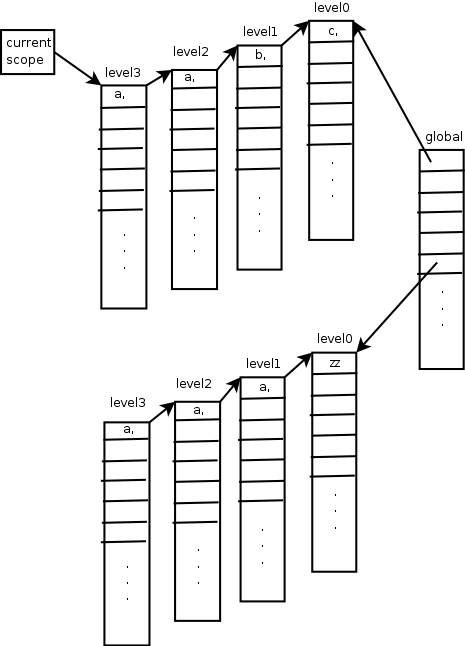
\includegraphics[scale=0.3]{symbol_table.png}


\subsection{Type Checking}
As we are using recursive-descent, it is possible to embed all our type checking inside the parser itself. Doing so we can essentially achieve a ``free'' traversal of the parse tree, at the expense of conflating the parser and possibly introduce extra complications. Or we could heed the advice of the SoftEng folks by keeping the two phases separate, and write some tree-walker functions that would take the parse tree and then perform all the type checking. We decided to take a hybrid approach: we would do all our type checking along with the parser, but we will not clutter our parser with any type checking code. This way, we get a free traversal and also keep our parser clean. \\

The way in which it was implemented is pretty neat: we simply create a do-function for each non-terminal. This do-function will receive as input a list of thunked\footnote{A thunk is an expression wrapped inside a lambda abstraction} functions to apply. We needed to thunk the functions, or else Scheme would actually evaluate the arguments when we called the do-function (since Scheme uses Applicative Order Evaluation). And since the functions are thunked, our do-function has the ability to do stuff before or after calling any function (for example, creating/deleting scope information). Needless to say, all of our do-functions are written manually so that we can fine-tune everything that is performed. For example, we are now able to output detailed error messages when we encounter a type error.  \\

There are several disadvantages to our approach. Firstly, writing a large amount of code takes a lot of time, and is also harder to debug. We can attest to this fact, as quite a lot of our development time was actually spent debugging our code rather than producing it. Secondly, although we do keep the parser code and type checking code separate, they are still being executed \emph{at the same time}. This means that if there is a parse error, we need to also ensure that our type checking does not get into a mangled state. The effects of this was mitigated through the use of an internal parser type called ALPHA, which essentially unifies with any type (and thus suppresses redundant error messages). Another problem with writing out the code manually is that now the do-functions are tightly coupled with the grammar - making a change to the grammar requires us to also change the corresponding do-function, which is pretty lame. \\

We mentioned above that we have a lot of code for type checking (actually, over 1000 lines). Naturally we considered whether we could automatically generate this code somehow, perhaps using attribute grammars. In order to do this, we would need to include type information in our CFG, and modify our parse functions to return a tuple of [AST,type], so that the calling function is able to perform the type checking. We would also need to modify our parser generator to be able to read this attribute grammar. However, we decided against this approach as we could not clearly see how to automate the type checking. Perhaps if given more time, we may decide to figure out how to automate our type checking but for now, we will have to surrender to manual labour. \\

In Assignment 1, we thought that we would have problems evaluating certain expressions since our parse tree is right-associative e.g. 18/9/3. However, it turned out that it was quite easy to fix. \\

\subsection{Code Generation}
This ``compiler'' generates Python code. In the finest sense of the word, NYAC is not really a compiler since it does not generate assembly code; rather, it should be called a translator. However, we decided to leave the name as it was for historical reasons (and it sounds better than NYAT). \\

When doing our planning for Assignment 3, we first considered using the sparc-cgen tool that was made available to us on the course website. Using sparc-cgen would be pretty easy and straightforward -- we already have our own intermediate representation, so all we would have to do is convert ours to match the format of sparc-cgen. However, after playing around with sparc-cgen for a while, we realised that it was quite limited in terms of features e.g. no support for floating point types. We also did not want to use any code that we did not write ourselves, thus we decided against using sparc-cgen. \\

We also considered generating SPARC assembly code manually. While that would be cool to do, it would also be very complicated as we would have to implement everything ourselves - register allocation, memory management, etc. And to add to that, time was against us so we probably would not have had enough time to implement everything that we wanted to in time for the deadline. From our experience in CS241, coding in assembly requires a lot of time consuming low-level details and so we wanted to bypass some of that if it was possible. \\

Thus we thought of implementing a virtual machine on the SPARC architecture and then generating code for our VM. But that would also require a lot of time in itself, so we decided to put that thought on hold. Then we thought, of using another VW instead of writing our own? We did some research and found several candidates available, the interesting ones being: Java, Lua, and Parrot. Of those three, we decided that Java would be the best candidate since it has a lot of features (eg. classes, garbage collection) and the Java Virtual Machine is available virtually everywhere\footnote{JAVA: write once, debug everywhere -- \emph{author unknown}}, including the undergrad computing environment. Thus we spent some time on reading about the JVM, and examining disassembled versions of class files using javap. We wrote a trivial prototype that translated a tiny subset of our code IR into a Java bytecode and were preparing to adopt it as our primary generator. \\

In the mean time, we noticed that someone\footnote{Holden Karau} posted on the course newsgroup and asked whether we could generate C and then use gcc to output assembly code, which was deemed fair game by Prof G. Cormack. That would certainly be a lot easier than generating Java byte-code, which was a very tedious thing to work with. \\

We were now considering generating high-level languages. After a bit of brainstorming, we thought of several possible languages: C, C++, Java, Python, and Ada?! Well, simply put ``generating'' Ada would be oversimplified, so that was out of the question. C++ would be suitable since it shares many features available to Ada and it also has templates, so we could possibly even implement generics. However, it does not have built-in support to handle nested procedures. After a bit of google-ing, we found some hacks to simulate the behaviour of nested procedures in C++, but the code was really ugly and we did not want to generate that sort of code. Java also does not support nested procedures, and the feature set available is basically very similar to C++. C is also quite similar to Ada, and indeed it even has support for nested procedures. However, it is also lacking many features in C++, such as the Standard Template Library. Furthermore, we thought that generating C/C++/Java would be very lame, and also we would not learn anything since we already know those languages. \\

Then we came to Python. Python is a multi-paradigm programming language with a fully dynamic type system, and uses automatic memory management. Thus we would not need to worry about generating any type information in our code or worry about garbage collection. In addition, there is support for nested functions, for classes, and also functional programming tools. Furthermore we were interested in learning Python, but never got the chance. Thus we could kill two birds with one stone by adopting Python as our output code. Indeed, we argue that generating Python is comparable to generating C/C++/Java, or even the IR for sparc-cgen, but it is considerably easier than manually generating Assembly. \\

While we have gained experience in using Python from this project, we do feel somewhat incomplete since we have not produced any assembly code (not to mention the fact that Python is interpreted). If we had more time on our hands, we would have linked to experiment with generating assembly and utilizing some of the theory shown to us in class. We were really interested in trying some compiler optimizations using Single Static Assignment (SSA) as our IR, as well as garbage collection. However, we deemed it higher priority to have something that works instead of a half-finished product.

\subsubsection{Code Generation Specifics}
For the most part, converting Ada code into Python was relatively straightforward. The expressions and functions were almost a direct translation, except that in the case of functions, Python sometimes requires an extra parameter called ``self''. ``If statements'', ``while statements'', ``for loops'', recursion, and named parameters are all supported by default in Python. In the case of ``for loops'', Python already has a ``range'' statement which greatly simplifies writing ``for loops'' (so we could do something like: ``for x in range(1,6)'', which in Ada would be equivalent to: ``for x in 1..5 loop''). \\

Although Python does not have support for ``blocks'' by default, we were able to simulate the effect by transforming ``blocks'' into local procedures, and then calling the procedure immediately after. However, we did encounter several speedbumps when generating certain features: access types, and ``exit when'' statements. By default, all variables (apart from primitives such as ``int'' and ``bool'') are references by default, and there does not exist something like a pointer per se. However, we were able to simulate pointers by making all our variables into dictionaries that only have one field called ``all''. This way, whenever we change the value of the object being ``pointed to'' by the pointer, the ``pointer'' gets updated as well. While this does allow us to support access types, there is no free lunch: the code is much uglier, and we would have to modify our ``for loops'' -- all our variables are now dictionaries so we cannot simply use the ``range'' function mentioned above to code our ``for loops''. Thus we had to write our own versions of the ``range'' function, and the corresponding reverse generator as well, which would be prepended to every file that we generated. \\

``Exit when'' statements, while not supported by default in Python, were rather simple to do. We chose to implement them using exceptions. Thus, whenever we have a ``named block'', we would wrap it in a try/except block, and create an exception corresponding to the name of the ``named block'' which does nothing when raised. Then, whenever we want to exit from this block, we raise the exception corresponding to the name of the block. This does achieve the correct behaviour, but it also results in much bloated code. While there may be more elegant solutions available, this method was the simplest to implement, so we are willing to live with it. \\

To implement quoted attributes such as 'Floor and 'Ceiling, we decided to simply use Python's math library. Thus in every generated file, we would import the math library. This does not cause any ``namespace pollution'', since in Python we must specify the full path when calling library functions (e.g. math.floor). In addition, we have taken extra precautions to avoid namespace collisions with Python built-in functions by always prepending an underscore to all of our function names (such names are not valid Ada identifiers, and thus cannot occur in valid Ada code). \\

When looking at our generated code, the observant reader will notice that we have quite a lot of ``pass'' statements. This is due to the fact that Python does not allow empty blocks i.e. each block must have at least one statement. Thus we chose to always insert a ``pass'' statement at the beginning of every block to fulfil this requirement. We admit that we have inserted ``pass'' statements unnecessarily in some cases. However, the view we take is that it is better to be safe than sorry, and also those ``pass'' statements do not incur much overhead during runtime. Similarly with ``exceptions'', we have always included a ``dummy'' exception in the event that the user did not specify any ``exceptions''.

Here is an example of all the boilerplate stuff generated by our compiler to implement the features discussed above: \\

\begin{alltt}
\verbatimtabinput[2]{headers.py}
\end{alltt}

\subsection{Testing}
Performing type checking involved handling numerous cases. In order to streamline our development process, we needed to ensure that whenever we implemented a new feature, the feature did indeed work, and that nothing else was broken in the process. Performing manual testing on our test cases quickly became tiresome, so we wrote a small script called run.sh. This script will run all of our testcases ($\ast$.ada) in the tests/ directory and write the results to the corresponding .out file, and then combine the original file as well as the results into a single file aptly called ``output''. In addition, it will also concatenate the a.out file into the output file as well. Thus, whenever we want to do some tests, we just need to run run.sh and then examine the output file. \\

It would also be cool if we could somehow diff the results, but due to the frequency of changes to our code that option is not feasible at the moment.

\subsubsection{Sample Programs}

Note: All of the following programs are available in our tests/correct directory

\begin{alltt}
INPUT FILE: default_values.ada
\verbatimtabinput[2]{correct/default_values.ada}
GENERATED CODE:
\verbatimtabinput[2]{correct/default_values.exe}
OUTPUT:
\verbatimtabinput[2]{correct/default_values.out}

INPUT FILE: dyn_default_values.ada
\verbatimtabinput[2]{correct/dyn_default_values.ada}
GENERATED CODE:
\verbatimtabinput[2]{correct/dyn_default_values.exe}
OUTPUT:
\verbatimtabinput[2]{correct/dyn_default_values.out}

INPUT FILE: exceptions1.ada
\verbatimtabinput[2]{correct/exceptions1.ada}
GENERATED CODE:
\verbatimtabinput[2]{correct/exceptions1.exe}
OUTPUT:
\verbatimtabinput[2]{correct/exceptions1.out}

INPUT FILE: factorial.ada
\verbatimtabinput[2]{correct/factorial.ada}
GENERATED CODE:
\verbatimtabinput[2]{correct/factorial.exe}
OUTPUT:
\verbatimtabinput[2]{correct/factorial.out}

INPUT FILE: fib.ada
\verbatimtabinput[2]{correct/fib.ada}
GENERATED CODE:
\verbatimtabinput[2]{correct/fib.exe}
OUTPUT:
\verbatimtabinput[2]{correct/fib.out}

INPUT FILE: fibrec.ada
\verbatimtabinput[2]{correct/fibrec.ada}
GENERATED CODE:
\verbatimtabinput[2]{correct/fibrec.exe}
OUTPUT:
\verbatimtabinput[2]{correct/fibrec.out}

INPUT FILE: primes.ada
\verbatimtabinput[2]{correct/primes.ada}
GENERATED CODE:
\verbatimtabinput[2]{correct/primes.exe}
OUTPUT:
\verbatimtabinput[2]{correct/primes.out}

INPUT FILE: mandelbrot.ada
Note: This program writes to standard output a pictorial representation of Mandelbrot with artificial colouring using a PPM format.
\verbatimtabinput[2]{correct/mandelbrot.ada}
GENERATED CODE:
\verbatimtabinput[2]{correct/mandelbrot.exe}
\end{alltt}

Output file converted to PNG: \\

\includegraphics[scale=1.0]{correct/brot.png}

\section{Afterword}
Having completed a substantial subset of Ada/CS, we feel wiser and more experienced. In addition, begin given this opportunity to develop a serious (to some degree) project, we are immensely gracious to those who have guided us in this journey, and special thanks goes to Prof. G Cormack for all his time and patience in answering our questions. \\

We would also like to say a word or two about the programming language that made it all possible for us. While developed with minimalistic thoughts in mind, Scheme has proven to be a powerful and sophisticated tool in software development. To illustrate some of the power of Scheme, we are somewhat proud to say that we have completed our entire compiler project in under 5000 lines\footnote{We could have had much less if we tried} of Scheme code, including comments and extra newlines thrown in for readability. We are quite confident that if we chose a language such as C++ or Java, our code base would have been 4 times larger (at least). We feel sorry that this language and so many others like it are overshadowed by the monomorphic mundane few and are thankful for the opportunity to know and exercise our minds and skills with it. \\

We look forward to challanges yet to overcome.

\begin{thebibliography}{99}

\bibitem{olsen82} Olsen, Whitehill 1982: \emph{Ada technology development at Irvine Computer Sciences Corporation}
\bibitem{davie81} Davie A.J.T, Morrison R. 1981: \emph{Recursive Descent Compiling}
\bibitem{fischer88} Fischer, Leblanc, Cytron 1988: \emph{Crafting a Compiler}
\bibitem{cooper04} Cooper D.K, Torczon L. 2004: \emph{Engineering a Compiler}
\bibitem{burke83} Burke G.M, Fisher A.G. 1983: \emph{A Practical Method for LR and LL Syntactic Error Diagnosis and Recovery}
\bibitem{ford02} Ford A.B 2002: \emph{Packrat Parsing: Simple, Powerful, Lazy, Linear Time}
\bibitem{ford04} Ford A.B 2004: \emph{Parsing Expression Grammars: A Recognition-Based Syntactic Foundation}
\bibitem{okasaki98} Okasaki C. 1998: \emph{FUNCTIONAL PEARLS: Even higher-order functions for parsing or Why would anyone ever want to use sixth-order function?}
\bibitem{meijer96} Meijer E. 1996: \emph{FUNCTIONAL PEARLS: Monadic Parsing in Haskell}
\bibitem{hutton92} Hutton G. 1992: \emph{Higher-Order Functions for Parsing}
\bibitem{swierstra96} Swierstra S.D, Duponcheel L 1996: \emph{Deterministic, Error-Correcting Combinator Parsers}

\end{thebibliography}

\end{document}
